\documentclass[12pt,a4paper]{article}
\usepackage[utf8x]{inputenc}
\usepackage{ucs}
\usepackage[MeX]{polski}
\usepackage{fancyhdr}
\usepackage{amsmath}
\usepackage{amsfonts}
\usepackage{amssymb}
\pagestyle{fancy}
\usepackage{enumerate}
\usepackage{listings}
\usepackage{subfig}
\usepackage[final]{pdfpages}

\begin{document}
\LARGE\centering Założenia projektowe\\
\large\centering Projekt realizowany w ramach kursu Wizualizacja Danych Sensorycznych na Politechnice Wrocławskiej\\
\vspace{5 mm}
\normalsize\flushleft\textbf{Tytuł Projektu:} Wizualizacja czujników rękawicy sensorycznej\\
\textbf{Autorzy:} Krzysztof Dąbek 218549, Dymitr Choroszczak 218627\\
\textbf{Kierunek:} Automatyka i Robotyka\\
\textbf{Specjalność:} Robotyka (ARR)\\
\textbf{Prowadzący:} dr inż. Bogdan Kreczmer\\
\textbf{Kurs:} Wizualizacja Danych Sensorycznych\\
\textbf{Termin zajęć:} pt 11:15\\
\vspace{5 mm}

\section{Opis projektu} \normalsize
Celem jest wizualizacja uproszczonego modelu dłoni na podstawie danych z rękawicy sensorycznej. 
Efektem końcowym jest przedstawienie orientacji dłoni oraz zgięcia palców w przestrzeni trójwymiarowej. \\
\vspace{1cm}
\subsection{Projekt skupia się na ukazaniu}
\begin{itemize}
\item Zgięcia trzech palców przez zmianę konfiguracji przegubów modelu
\item Siły nacisku opuszków na powierzchnię poprzez zmianę koloru i/lub rozmiaru obiektów sferycznych, umieszczonych na zakończeniach skrajnych przegubów modelu
\item Orientacji dłoni względem wektora grawitacji
\end{itemize}
\subsection{Specyfikacja urządzenia (rękawicy sensorycznej)}
\begin{itemize}
\item Na opuszkach palców zamontowane zostaną czujniki siły nacisku FSR-400. Spadek rezystancji przy przyłożonej sile pozwala zmierzyć siłę nacisku.
\item Do wykrycia zgięcia stawów międzypaliczkowych bliższych oraz stawu międzypaliczkowego kciuka zastosowane zostaną czujniki ugięcia - flexsensory firmy Sparkfun. Zgięcie tych sensorów powoduje wzrost rezystancji.
\item Akcelerometr LSM303DLHC, znajdujący się na płytce Discovery zostanie użyty do określenia orientacji rękawicy względem wektora grawitacji.
\item Powyższe elementy nie zapewniają bardzo precyzyjnych pomiarów, ale zostały wybrane ze względu na cenę i charakter projektu, w którym zostaną zastosowane.
\item Jako urządzenie nadawcze Bluetooth posłuży moduł HC-06 z interfejsem UART podłączony do płytki Discovery.
\end{itemize}

\subsection{Funkcjonalności aplikacji}
Zostanie stworzona aplikacja okienkowa do wizualizacji napisana w języku C++ z użyciem biblioteki Qt.\\
\begin{itemize}
\item W aplikacji zostanie stworzony uproszczony model dłoni ludzkiej o trzech palcach, przedstawiony przegubami manipulatorów.
\item Połączenie z rękawicą sensoryczną za pomocą wybranego portu magistrali szeregowej komputera.
\item Połączenie z rękawicą sensoryczną przez Bluetooth.
\item Kalibracja i skalowanie modelu dłoni.
\item Uruchomienie i zatrzymanie pomiarów, wykonanie pojedynczego pomiaru.
\item Wyświetlanie liczbowo wyników pomiarów i możliwość zapisania ich do pliku.
\end{itemize}

Projekt zostanie połączony z innym realizowanym w ramach kursu Roboty Mobilne 1. Dane do wizualizacji będą wysyłane przez płytkę wykonanej rękawicy sensorycznej.

\newpage
%Rozpisać na kolejne tygodnie
\section{Harmonogram}
\begin{itemize}
\item (31.03.2017) Uruchomienie i przetestowanie pętli USB$\rightarrow $UART$\rightarrow $USB w celu symulacji danych sensorycznych 
\item (14.04.2017) Stworzenie struktur danych wykorzystywanych w aplikacji (przeguby, manipulatory, scena)
\item (14.04.2017) Stworzenie okna programu i wszystkich jego funkcjonalności
\item (23.04.2017) Wczytywanie i dekodowanie danych z rękawicy sensorycznej
% Wstępne rezultaty
\item (05.05.2017) Stworzenie uproszczonego modelu kośćca dłoni
\item (05.05.2017) Stworzenie elementów potrzebnych do wizualizacji czujników nacisku (kolorowe sfery na opuszkach)
\item (14.05.2017) Poruszanie przegubami na podstawie odczytów z tensorów i kinematyki prostej manipulatorów
\item (14.05.2017) Zmiana koloru i/lub wielkości sfer na podstawie odczytów z czujników nacisku
%Rezultaty prawie końcowe
\item (26.05.2017) Obrót modelu na podstawie akcelerometru
\item (26.05.2017) Komunikacja przez Bluetooth
\item (02.06.2017) Testy aplikacji
\item (11.06.2017) Naprawianie błędów
\item (11.06.2017) Wizualne ulepszenie aplikacji
%Rezultaty końcowe
\end{itemize}

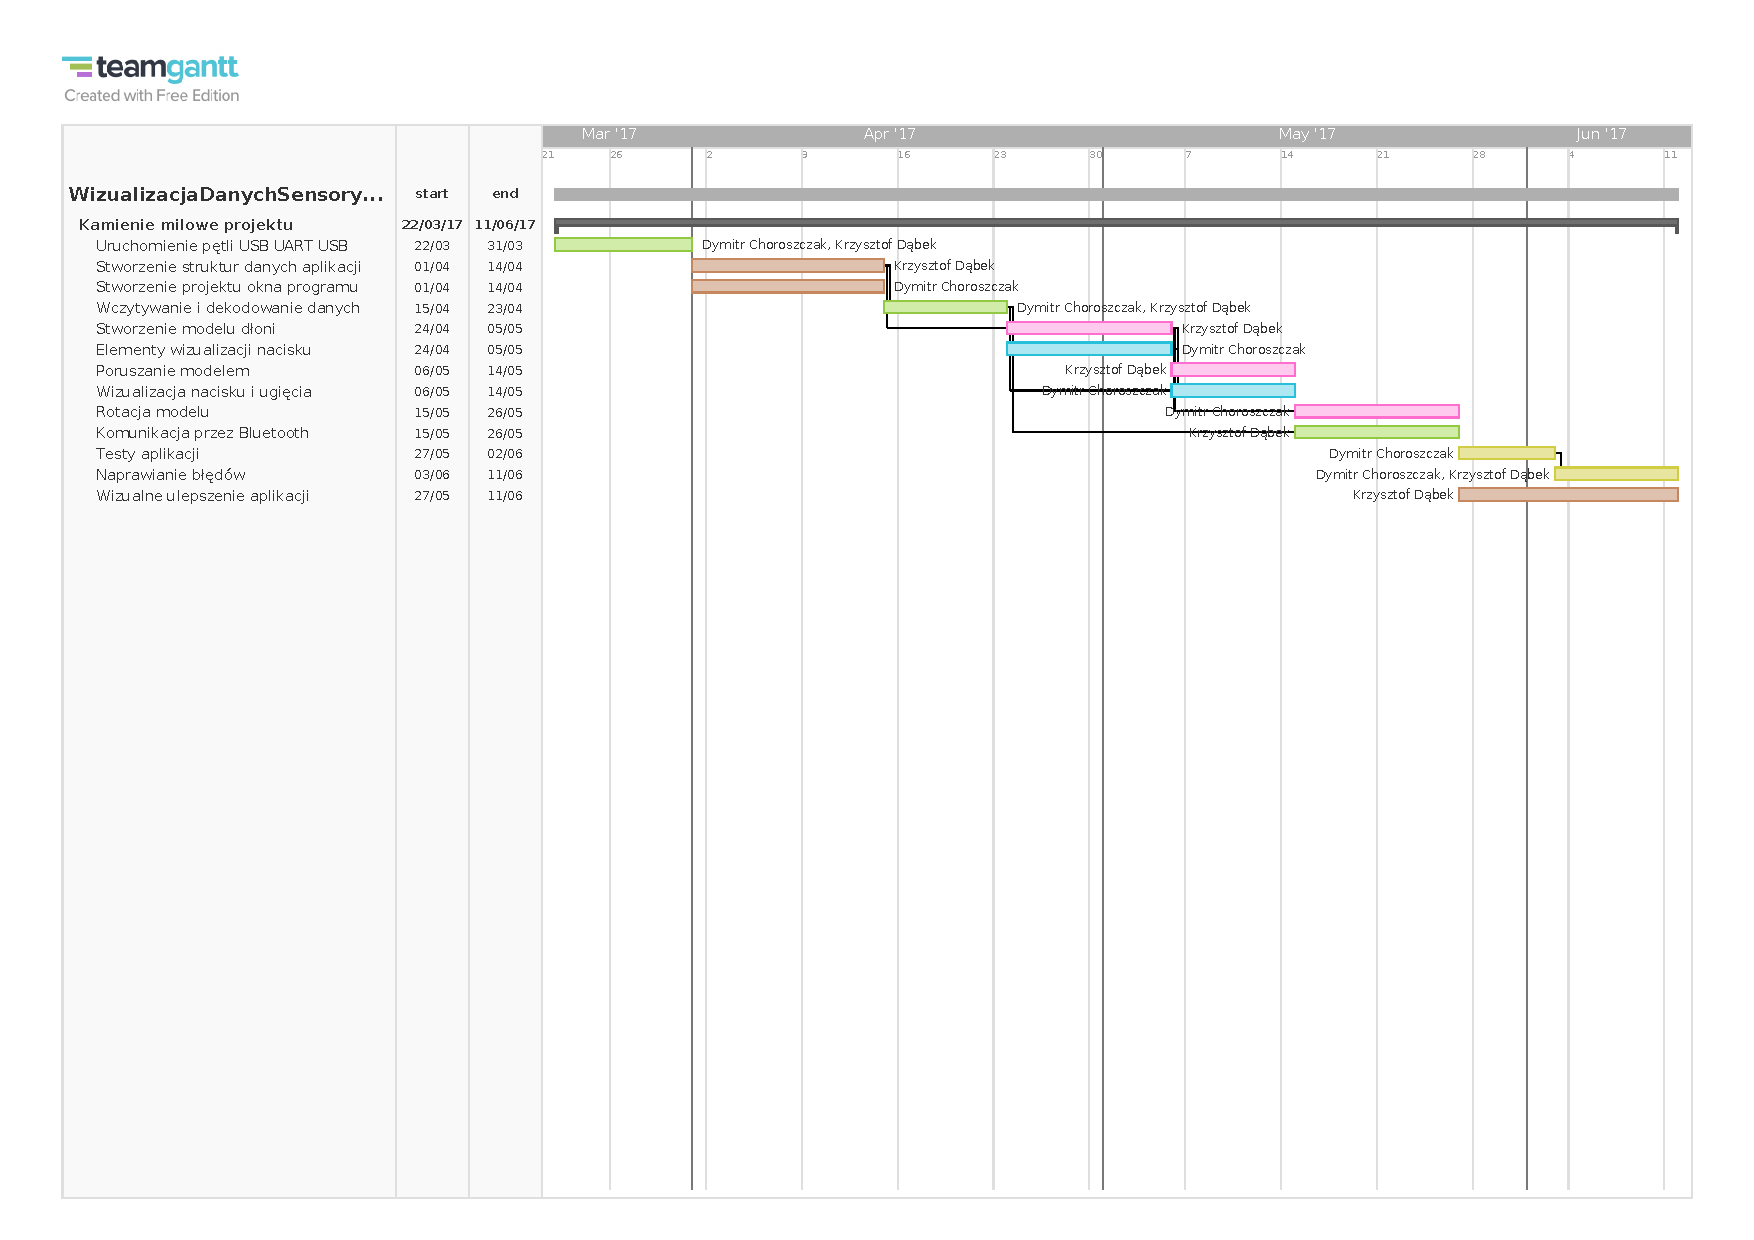
\includepdf[pages={-},angle=-90]{Gantt.pdf}

\end{document}